\documentclass{beamer}
 
\usepackage[utf8]{inputenc}
\usepackage[brazil]{babel} % pacote portugues brasileiro
\usepackage{textpos}
\usepackage{hyperref}
\definecolor{blue(pigment)}{rgb}{0.2, 0.2, 0.6}
\hypersetup{
    colorlinks=true,
    linkcolor=blue(pigment),
    filecolor=magenta,      
    urlcolor=cyan,
}

\usepackage{verbatim}
\usetheme{Montpellier}
\usecolortheme{rose}
% \graphicspath{{../../../2021-1/DesWebBasico/aulas/fig/}}
% Layout da pagina
\hypersetup{pdfpagelayout=SinglePage}
 
%Information to be included in the title page:
\title[HTML]{HTML - parte 2}
 \subtitle{Disciplina: Desenvolvimento de Sistemas com PHP}
\author{Juliana C. Silva}
\institute{Universidade Positivo}
%\date{10 de março de 2021}
\definecolor{UniGray}{RGB}{192,192,192}
\definecolor{nGray}{RGB}{220,220,220}

\setbeamercolor{block title}{use=structure,bg=UniGray}
\setbeamercolor{block body}{use=structure,bg=nGray}
\setbeamersize{text margin left=25pt,text margin right=25pt}
\setbeamertemplate{navigation symbols}{}%remove navigation symbols
 
% Configurando layout para mostrar codigos C++
\usepackage{listings}
\lstset{
  language=HTML,
  basicstyle=\ttfamily\small, 
  keywordstyle=\color{blue}, 
  stringstyle=\color{red}, 
  commentstyle=\color{red}, 
  extendedchars=true, 
  showspaces=false, 
  showstringspaces=false, 
  numbers=left,
  numberstyle=\tiny,
  breaklines=true, 
  backgroundcolor=\color{green!10},
  breakautoindent=true, 
  captionpos=b,
  xleftmargin=0pt,
}

\begin{document}
%------------------------------------------------------------------------------------------
\frame{\titlepage}
 
\addtobeamertemplate{frametitle}{}{%
\begin{textblock*}{100mm}(.8\textwidth,-1.45cm)
%\includegraphics[height=0.8cm,width=2.5cm]{fig/logo_unicesumar.png}
\end{textblock*}
}

%-----------------------------------------------------------------------------------------
\section{Contexto}
\begin{frame}{Na última aula...}
  \begin{enumerate}
   \item Páginas WEB
   \item Tags HTML
   \item Estrutura de uma página WEB
  \end{enumerate}
\end{frame}
%------------------------------------------------------------------------------------------
\begin{frame}
\frametitle{Na aula de hoje} 
\tableofcontents 
\end{frame}
%---------------------------------------------------------------------------------
\begin{frame}{Estrutura página WEB}
		\begin{center}
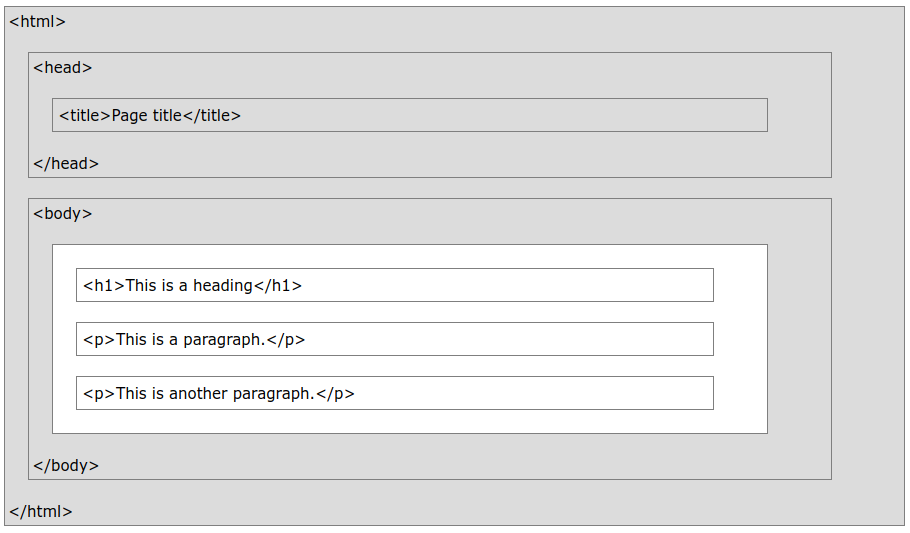
\includegraphics[height=0.65\paperheight]{fig/aula2/html_page.png} \\
    		\tiny \textbf{Fonte:} \cite{wschool2021html}.
		\end{center}
\end{frame}
%-------------------------------------------------------------------------------
\begin{frame}{Estrutura página WEB}
		\begin{center}
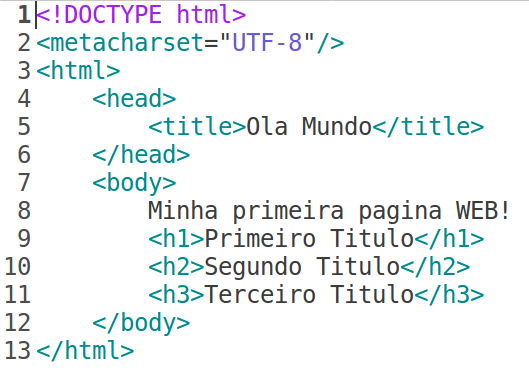
\includegraphics[height=0.65\paperheight]{fig/aula2/html1.png} \\     		
\tiny \textbf{Fonte:} \cite{wschool2021html}.
		\end{center}
\end{frame}
%---------------------------------------------------------------------------------
\section{Listas}
\begin{frame}{Tags HTML - Listas}
  Listas são utilizada em diversas ocasiões em uma página HTML;
  \begin{itemize}
   \item A apresentação de itens do um assunto (como esse slide);
   \item Estruturação de novos componentes (como um menu);
  \end{itemize}
   Existem três tipos de listas no HTML:
  \begin{enumerate}
   \item Listas ordenadas;
    \item Listas não ordenadas;
    \item Listas de definições;
 \end{enumerate}
 Também é possível criar listas aninhadas.
\end{frame}
%---------------------------------------------------------------------------------
\begin{frame}{Lista ordenada}
  \begin{columns}
    \begin{column}{0.45 \textwidth}
     \begin{itemize}
      \item Cria uma lista que segue uma sequência numérica;
       \item Utiliza a tag $<$ol$>$ (\textit{ordered list});
       \item Cada item da lista é expresso entre a tag $<$li$>$ 
      (\textit{list item});
     \end{itemize}
    \end{column}
    \begin{column}{0.5\textwidth}
     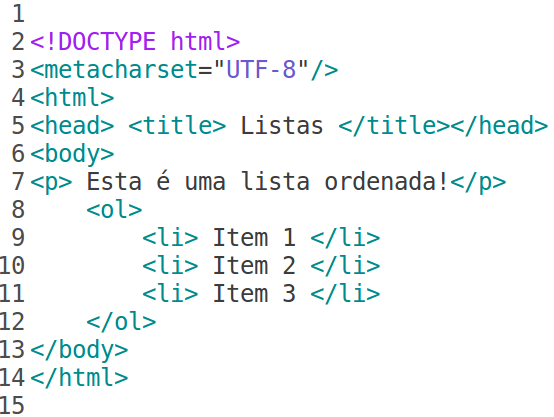
\includegraphics[height=0.45\paperheight]{fig/aula2/html2.png}
    \end{column}
  \end{columns}
\end{frame}
%---------------------------------------------------
\begin{frame}{Lista desordenada}
  \begin{columns}
    \begin{column}{0.45 \textwidth}
     \begin{itemize}
      \item Cria uma lista que não segue uma sequência.
       \item Utiliza a tag $<$ul$>$ (\textit{unordered list});
       \item Cada item da lista é expresso entre a tag $<$li$>$ 
      (\textit{list item});
     \end{itemize}
    \end{column}
    \begin{column}{0.5\textwidth}
     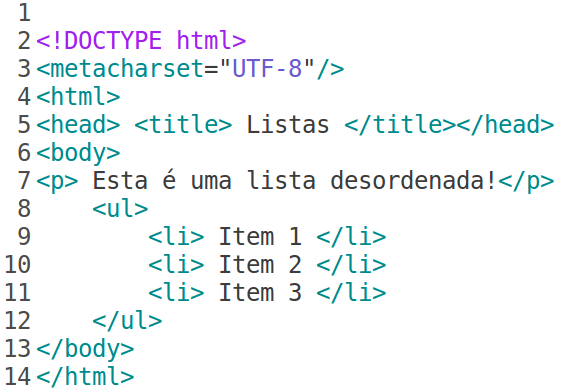
\includegraphics[height=0.45\paperheight]{fig/aula2/html3.png}
    \end{column}
  \end{columns}
\end{frame}
%---------------------------------------------------
\begin{frame}{Lista de definição}
  \begin{columns}
    \begin{column}{0.45 \textwidth}
     \begin{itemize}
      \item Cria uma lista que define algum termo.
       \item Utiliza a tag $<$dl$>$ (\textit{definition list});
       \item Um termo é representado pela tag $<$dt$>$ 
(\textit{definition term});
       \item A definição é representada pela tag $<$dd$>$ 
      (\textit{definition definition});
       \item Uma $<$dt$>$ pode ter uma ou mais $<$dd$>$;
     \end{itemize}
    \end{column}
    \begin{column}{0.5\textwidth}
     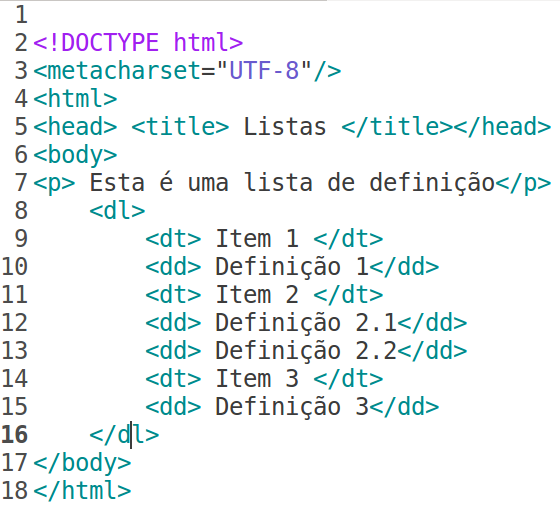
\includegraphics[height=0.55\paperheight]{fig/aula2/html4.png}
    \end{column}
  \end{columns}
\end{frame}
%-------------------------------------------------------
%-------------------------------------------------------------
\begin{frame}{Listas aninhadas}
  \begin{columns}
    \begin{column}{0.45 \textwidth}
     \begin{itemize}
      \item Um item de uma lista pode se tornar uma nova lista;
       \item Essa estrutura representa uma sub lista de uma lista 
principal;
     \end{itemize}
    \end{column}
    \begin{column}{0.5\textwidth}
     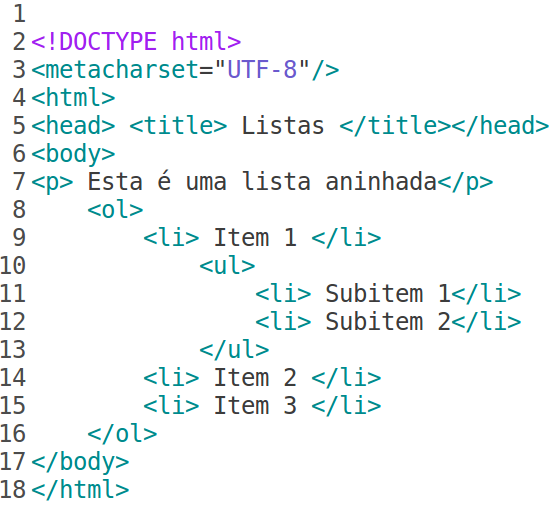
\includegraphics[height=0.55\paperheight]{fig/aula2/html5.png}
    \end{column}
  \end{columns}
\end{frame}
%-------------------------------------------------------------
\section{Âncoras (Links)}
\begin{frame}{Links}
  
  \begin{columns}
    \begin{column}{0.45 \textwidth}
  
      \begin{itemize}
      \item Permitem a movimentação entre páginas;
       \item Utilizado com a tag $<$a$>$;
       \item \textbf{href:} endereço da página na qual o link 
aponta; 
       \item mailto: abre a interface para envio de e-mail;
       \item \#id: uma parte específica da página;
       \item Download: link é um download;
     \end{itemize}
    \end{column}
    \begin{column}{0.5\textwidth}
     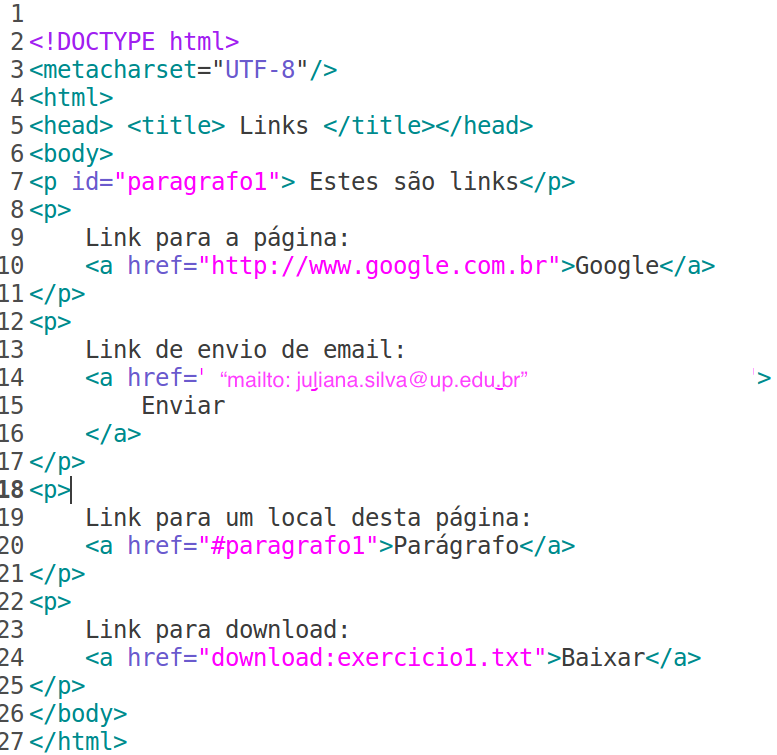
\includegraphics[height=0.6\paperheight]{fig/aula2/html6.png}
    \end{column}
  \end{columns}
\end{frame}
%--------------------------------------------------------------------------
\begin{frame}{Links}
  Parâmetros de link:
     \begin{itemize}
      \item \textbf{target:} especifica onde abrir o novo documento
       \item \_blank: abre em uma nova janela;
       \item \_self: abre onde o documento atual está (default); 
     \end{itemize}
     
     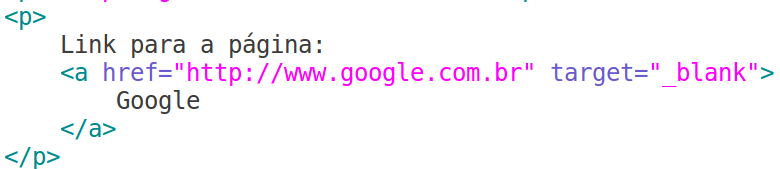
\includegraphics[height=0.25\paperheight]{fig/aula2/html7.png}
\end{frame}
%---------------------------------------------------------------------------
\section{Imagens}
\begin{frame}{Imagens}
  Adicionando imagens na página
  \begin{columns}
    \begin{column}{0.45 \textwidth}
     \begin{itemize}
      \item Representada pela tag $<$img$>$
       \item Parâmetros
      \begin{itemize}
	 \item \textbf{src:} aponta o caminho da imagem;
	 \item \textbf{alt:} indica um texto que substitui a imagem;
	 \item \textbf{title:} apresenta informação adicional sobre a 
imagem (tootip);
      \end{itemize}
    
     \end{itemize}
    
    \end{column}
    \begin{column}{0.5\textwidth}
     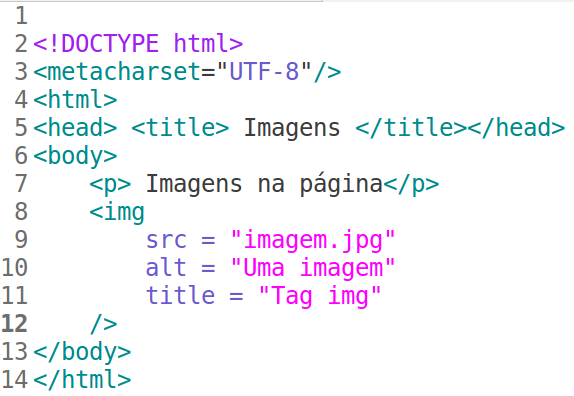
\includegraphics[height=0.45\paperheight]{fig/aula2/html8.png}
    \end{column}
  \end{columns}
\end{frame}
%---------------------------------------------------------------------------
\begin{frame}{Imagens}
  Adicionando imagens como links na página

     \begin{itemize}
      \item Você pode utilizar uma imagem como link
       \item Basta adicionar a tag $<$img$>$ dentro da tag $<$a$>$
     \end{itemize}
   

     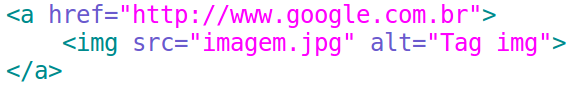
\includegraphics[height=0.15\paperheight]{fig/aula2/html9.png}
\end{frame}
%---------------------------------------------------------------------------
\begin{frame}{Elementos: Block}
  Elementos Block
     \begin{itemize}
      \item Elementos que “sempre” são renderizados no começo de
uma nova linha;
     \end{itemize}
 
 Elementos Block em HTML
  \vspace{0.3cm}
 \begin{center}
     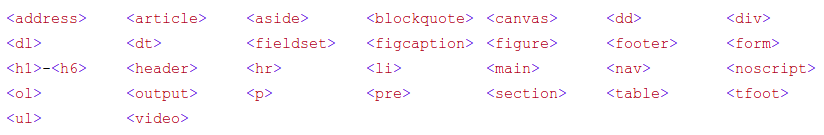
\includegraphics[height=0.18\paperheight]{fig/aula2/html12.png}
   \end{center}

\end{frame}
%---------------------------------------------------------------------------
\begin{frame}{Elementos: Inline}
  Elementos Inline
     \begin{itemize}
      \item Elementos que “sempre” são renderizados na mesma linha,
ao término de um elemento anterior;
     \end{itemize}
 
 Elementos InLine em HTML
 \vspace{0.3cm}
 \begin{center}
     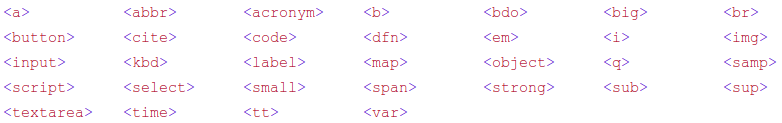
\includegraphics[height=0.18\paperheight]{fig/aula2/html13.png}
   \end{center}
\end{frame}
%---------------------------------------------------------------------------
\begin{frame}{Div}
  \begin{columns}
    \begin{column}{0.45 \textwidth}
      \small
     \begin{itemize}
       \item Permite o agrupamento de um conjunto de elementos em uma
box block-level;
       \item Cada conteúdo de uma div será apresentado em uma nova
linha;
       \item Esse comportamento pode ser alterado com CSS;
       \item Melhora a organização do código;
       \item É permitido colocar qualquer elemento dentro de uma div;
     \end{itemize}
    \end{column}
    
    \begin{column}{0.5\textwidth}
     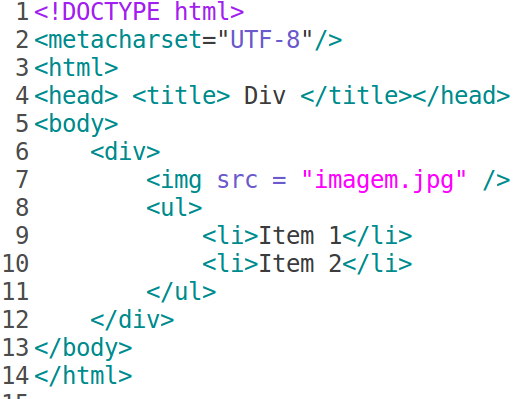
\includegraphics[height=0.5\paperheight]{fig/aula2/html14.png}
    \end{column}
  \end{columns}
\end{frame}
%--------------------------------------------------------------------
\section{Agrupando elementos}
\begin{frame}{Tag - Header}
  \begin{columns}
    \begin{column}{0.4 \textwidth}
      \small
      \begin{itemize}
	\item Utilizado para representar o cabeçalho de um documento ou seção;
	 \item Exemplo: cabeçalho de uma página;
      \end{itemize}
    \end{column}
    \begin{column}{0.55\textwidth}
     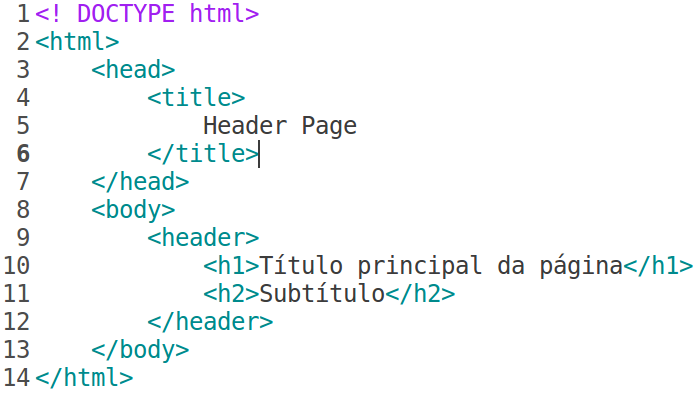
\includegraphics[height=0.4\paperheight]{fig/aula2/html15.png}
    \end{column}
  \end{columns}
\end{frame}
%---------------------------------------------------------------------------
\begin{frame}{Figure}
    \begin{columns}
    \begin{column}{0.4 \textwidth}
      \small
     \begin{itemize}
      \item Marcação de uso específico para a inserção de uma figura;
       \item Utilizado em conjunto com a tag $<$img$>$;
       \item Pode ser utilizado junto à tag $<$figcaption$>$ para 
adicionar uma descrição à imagem;
     \end{itemize}
    \end{column}
    
    \begin{column}{0.55\textwidth}
     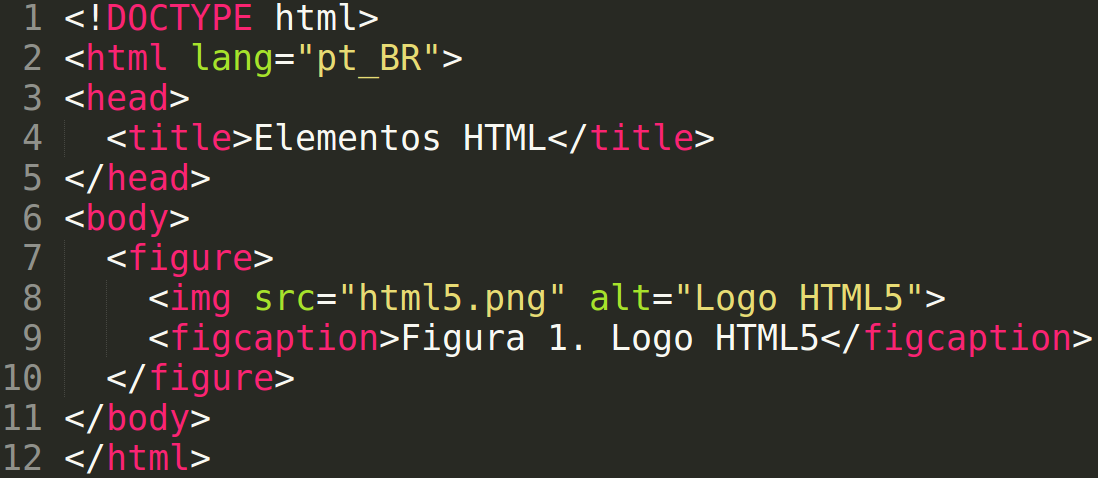
\includegraphics[height=0.3\paperheight]{fig/aula2/aula4_1.png}
    \end{column}
  \end{columns}
\end{frame}
%-------------------------------------------------------------------------------
\begin{frame}{Footer}
    \begin{columns}
    \begin{column}{0.4 \textwidth}
      \small
     \begin{itemize}
      \item Utilizado para representar o rodapé de um documento;
       \item Geralmente é utilizado para descrever informações de autoria 
para página;
     \end{itemize}
    \end{column}
    
    \begin{column}{0.55\textwidth}
     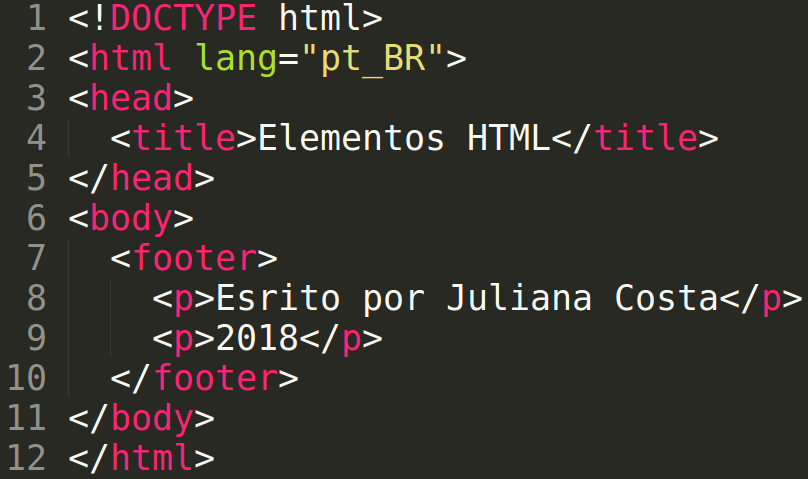
\includegraphics[height=0.4\paperheight]{fig/aula2/aula4_2.png}
    \end{column}
  \end{columns}
\end{frame}
%-------------------------------------------------------------------------------
\begin{frame}{Tabelas}
       \small
  Utilizada para tabular informações;\\
  \textbf{Exemplo:} relatório financeiro, programação de TV e resultados de 
esportes;
    \begin{columns}
    \begin{column}{0.5 \textwidth}
 
     \begin{itemize}
      \item $<$table$>$: cria e delimita o conteúdo de uma tabela;
       \item $<$tr$>$: delimita o conteúdo de uma linha 
       \item $<$td$>$: cria cada célula de uma linha;
       \item $<$th$>$: cria uma célula de cabeçalho;
     \end{itemize}
    \end{column}
    
    \begin{column}{0.45\textwidth}
     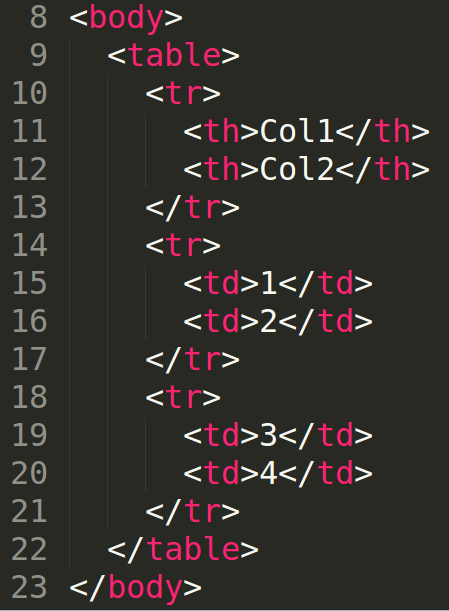
\includegraphics[height=0.5\paperheight]{fig/aula2/aula4_3.png}
    \end{column}
  \end{columns}
  
  \tiny{Não deve ser utilizada para determinar layout (tableless);}
\end{frame}
%-------------------------------------------------------------------------------
\begin{frame}{Tabelas}
    \begin{columns}
    \begin{column}{0.5 \textwidth}
      \small
     \begin{itemize}
      \item $<$thead$>$: delimita a primeira linha (geralmente o 
cabeçalho);
       \item $<$tbody$>$: delimita o conjunto de linhas de dados;
       \item $<$tfoot$>$: delimita a última linha (geralmente o rodapé ou 
resultados finais);
     \end{itemize}
    \end{column}
    
    \begin{column}{0.5\textwidth}
     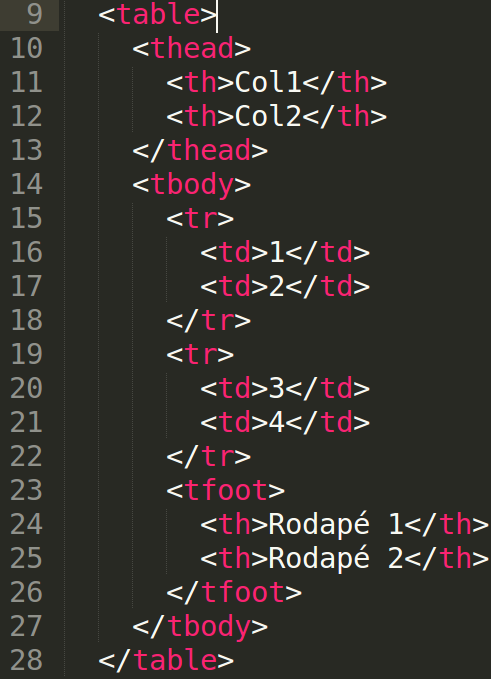
\includegraphics[height=0.6\paperheight]{fig/aula2/aula4_4.png}
    \end{column}
  \end{columns}
\end{frame}
%-------------------------------------------------------------------------------
\begin{frame}{Tabelas}
    \begin{columns}
    \begin{column}{0.5 \textwidth}
      \small
     \begin{itemize}
       \item \textcolor{red}{rowspan: mescla uma quantidade de linhas a partir 
	 de uma célula};
      \item colspan: mescla uma quantidade de colunas a partir de uma 
célula;
     \end{itemize}
    \end{column}
    
    \begin{column}{0.5\textwidth}
     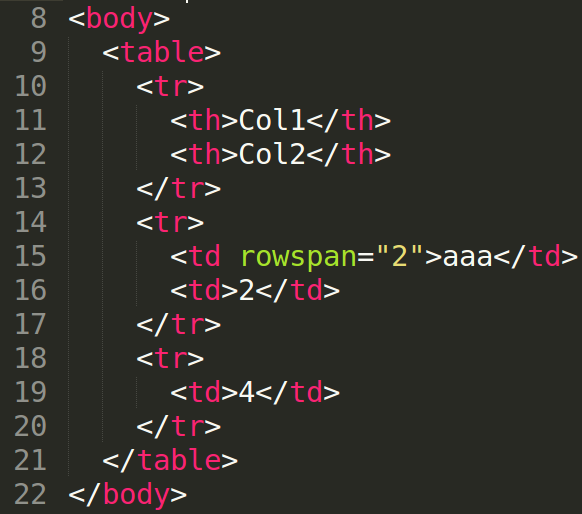
\includegraphics[height=0.5\paperheight]{fig/aula2/aula4_5.png}
    \end{column}
  \end{columns}
\end{frame}
%-------------------------------------------------------------------------------
\begin{frame}{Tabelas}
    \begin{columns}
    \begin{column}{0.5 \textwidth}
      \small
     \begin{itemize}
       \item rowspan: mescla uma quantidade de linhas a partir 
	 de uma célula;
      \item \textcolor{red}{colspan}: mescla uma quantidade de colunas a partir 
	de uma célula;
     \end{itemize}
    \end{column}
    
    \begin{column}{0.5\textwidth}
     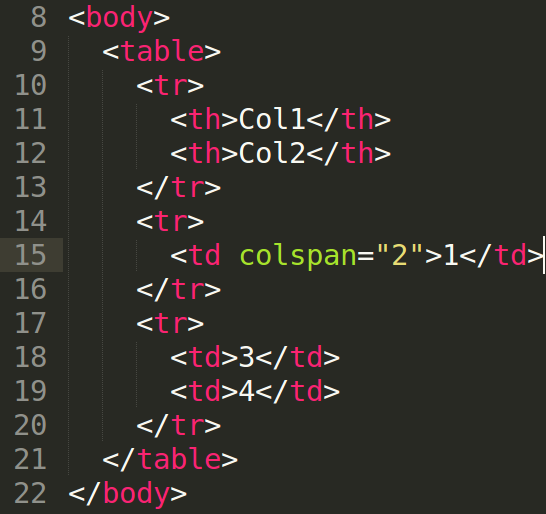
\includegraphics[height=0.5\paperheight]{fig/aula2/aula4_6.png}
    \end{column}
  \end{columns}
\end{frame}
%-----------------------------------------------------------------------
\section{Atividades}
\begin{frame}{Atividade I - Entrega via Blackboard}
\small
Desenvolva uma página WEB representando a Home de uma empresa (tipo de empresa é de livre escolha do aluno);

\begin{enumerate}
 \item Crie a página "index.html"
  \item Escreva um texto simples no topo da página contendo o nome da página.
  \item Inclua na página “index.html” um item que será utilizado para encaminhar o usuário para a página de contato com um link para a página “Atendimento”. 
  \item Inclua na página “index.html” um item que será utilizado para 
entrar na área de acesso restrito, com um link para a página "Login"
  \item Inclua na página "index.html" uma lista das opções de navegação: a) Quem somos b) Produtos c) Nossa história d) Serviços e) Equipe 
  \item Inclua na página uma divisão (div) com as principais informações (novidades) da empresa, utilize um cabeçalho "h1" para o título das informações e, um cabeçalho "h2" texto das novidades.
\end{enumerate}

\end{frame}
%---------------------------------------------------------------------------------
\section{Leitura recomendada}
\begin{frame}{Leitura complementar}
 Para mais informações sobre HTML5, leia:\\
 \begin{columns}
   \begin{column}{0.4\textwidth}
     HTML5 - Embarque imediato\\ 
      \cite{flatschart2011html}
   \end{column}
   \begin{column}{0.3\textwidth}
    \begin{center}
  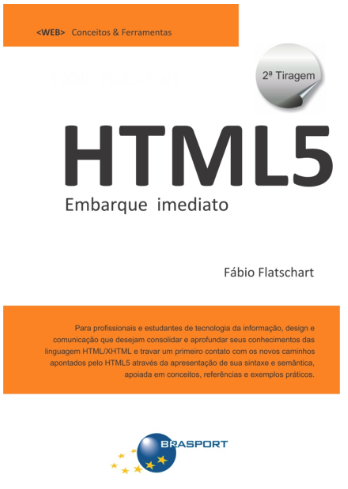
\includegraphics[height=0.5\paperheight]{fig/aula2/flatschart2014html.png} \\
 \end{center}
   \end{column}
 \end{columns}
\end{frame}
%----------------------------------------------------------------
\section{Referências}
\begin{frame}{Referências}%[allowframebreaks]
\frametitle{Referências}
\small
\begin{center}
\tiny
\bibliographystyle{apalike}
\bibliography{ref_aula}
\end{center}
\end{frame}
 
\end{document}
